\chapter{Pointingmodell für eine große Abweichung zur optischen Achse}
\label{ch:pointing}
Das Pointing von Teleskopen beschäftigt sich damit, dass das Teleskop so ausgerichtet wird, wie es erwünscht ist. Häufig ist das Problem, dass die eingestellte Position nicht exakt mit der gewünschten Position übereinstimmt. Gründe dafür können Fehler in der Präzision oder auch die Elastizität einzelner Bauteile sein. Im Fall der Sky-CCD des MST-Prototypen liegt es wie in Abschnitt \ref{se:cameras} beschrieben an der zentralen Befestigung die zu einem größeren Winkel zur optischen Achse führt. Da man die aufgenommen Daten mit den Bekannten Postionen am Himmel vergleichen kann, kann man versuchen ein Modell zu finden, welches die Fehler verkleinert oder im Idealfall sogar eliminiert.

\section{Koordinaten}
Das MST benutzt ein Koordinatensystem aus zwei Winkeln, welches den Kugelkoordinaten ähnelt. Der Azimutwinkel ($az$) beschreibt die Auslenkung in der Ebenen und läuft von $-180^{\circ}$ bis $180^{\circ}$, wobei es für $az=0^{\circ}$ in Richtung Norden ausgerichtet ist. Der Elevationswinkel $el$ läuft von $0^{\circ}$ bis $90^{\circ}$ wobei $el=90^{\circ}$ dem Zenit entspricht. Hier wird zudem die Konvention benutzt, dass Nordrichtung der x-Richtung, die Westrichtung der y-Richtung und die Zenitrichtung der z-Richtung entspricht.
\begin{figure}[htbp]
\centering
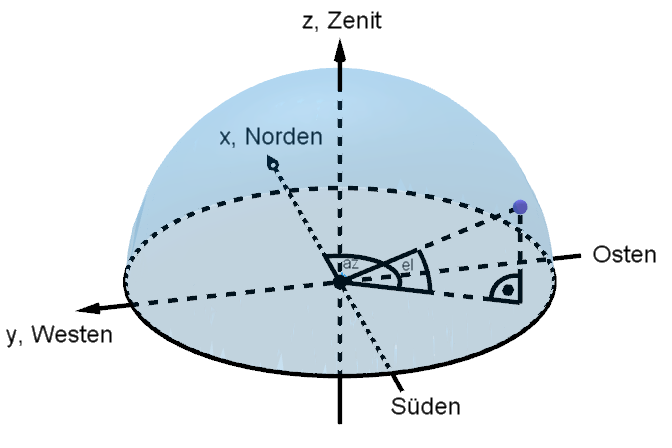
\includegraphics[width=0.7\textwidth]{Images/coordinates.png}
\caption{Die verwendeten Koordinaten}
\label{img:coordinates}
\end{figure}

\section{Entwicklung von Pointingmodellen}
Da man das Teleskop so ausrichten will, dass man die gewünschte Position vorgibt (Koordinaten der CCD- Index C) und dann die Koordinaten am Drive (Index D) einstellt, sucht man nach Funktionen, die die Koordinaten des Drives in Abhängigkeit von den gewünschten Koordinaten beschreibt. \\
In der Regel haben Teleskope so geringe Abweichungen zwischen eingestellter und tatsächlicher Position, dass sich diese Abweichungen als Funktionen schreiben lassen, die in den relevanten Parametern entwickelt werden können.
\begin{equation}
az_D=az_c+\Delta_{az}=az_C+\tilde{f}_{az}\left(az_c,el_c,\vec{q}\right)
\end{equation}
\begin{equation}
el_D=el_c+\Delta_{el}=el_C+\tilde{f}_{el}\left(az_c,el_c,\vec{q}\right)
\label{eq:pointingZero}
\end{equation}
Da die Sky-CCD des MST-Prototyps einen größeren Winkel ($\mathcal{O}\left(10^{\circ}\right)$) zur optischen Achse hat, lässt sich das Entwicklungsverfahren hier nicht anwenden. Stattdessen wird versucht, die einzustellende Position anhand geometrischer Überlegungen in Abhängigkeit der wahren Position vorherzusagen. Man versucht also Funktionen zu finden, die nur von den wahren Koordinaten und einem teleskopsspezifischen Parametersatz abhängen.
\begin{equation} 
az_D=f_{az}(az_C,el_C)
\end{equation}
\begin{equation}
el_D=f_{el}(az_C,el_C)
\label{eq:pointingprinciple}
\end{equation}

\section{Pointingmodell mit zwei Parametern}
\subsection{Vorhersage der CCD-Koordinaten in Abhängigkeit der Drive-Koordinaten}
Zunächst soll ein Pointingmodell mit zwei Parametern entwickelt werden, bei dem das Drivesystem in der Parkposition ($el_D=0,az_D=0$) in eine andere Richtung zeigt als die CCD-Kamera ($el_C=el_0,az_C=az_0$). Die beiden Positionen lassen sich auch durch zwei kartesische Richtungsvektoren $\vec{r_D}$ und $\vec{r_C}$ beschrieben. Ausgehend von dieser Startposition wird das Teleskop beziehungsweise die Vektoren $\vec{r_D}$ und $\vec{r_C}$ durch orthogonale Transformationen in die gewünschte Position gebracht wird. Als Parkpostion für das Drive-System erhält man mit den oben genannten Bedingung folgenden karthesischen Vektor:
\begin{equation}
\vec{r}_D^0=\left(\begin{array}{c} 1 \\ 0 \\ 0 \end{array}\right).
\label{eq:startDrive}
\end{equation}
Durch eine Drehung um die y-Achse mit dem Winkel $el$ und anschließender Drehung die z-Achse um den Winkel $az$ lässt sich aus dieser Startposition jeder Punkt auf der Einheitskugel erreichen. Die beiden Drehungen lassen sich zu einer Transformation $T(az,el)$ zusammenfassen:
\begin{equation}
T(az,el)=R_z(az)R_y(el)=
\left(\begin{array}{ccc} \cos(az) & \sin(az) & 0 \\ -\sin(az) & \cos(az) & 0 \\ 0 & 0 & 1\end{array}\right)
\left(\begin{array}{ccc} \cos(el) & 0 &-\sin(el) \\0 & 1 & 0\\ \sin(el) & 0 & \cos(el) \end{array} \right)
\end{equation}\\
\begin{equation}
T(az,el)=\left(\begin{array}{ccc} \cos(az)\cos(el) & \sin(az) &-\cos(az)\sin(el) \\-\cos(el)\sin(az) & \cos(az) & \sin(az)\sin(el)\\ \sin(el) & 0 & \cos(el) \end{array} \right).
\label{eq:TransformMat}
\end{equation}\\
Unter der Annahme, dass die Kamera von vornherein in eine andere Richtung als das Drive-System zeigt, lässt sich mit dieser Transformtion $T(az0,el0)$ aus der Startpostion des Drives die Startposition der Kamera bestimmen:
\begin{equation}
\vec{r}_C^0=T(az_0,el_0)\vec{r}_D^0=\left(\begin{array}{c} \cos(az_0)\cos(el_0) \\ -\cos(el_0)\sin(az_0) \\ \sin(el_0) \end{array}\right).
\label{eq:startCCD}
\end{equation}
Da hier angenommen wird, dass der Winkel zwischen der optischen Achse des Teleskops und der Kamera fest ist, sind $az_0$ und $el_0$ Konstanten. Wendet man nun die gleiche Transformation $T(az_D,el_D)$ mit den Koordinaten des Teleskops als Argumente auf beide Startvektoren an, so erhält man für jedes Koordinatenpaar des Drives die zugehörigen Koordinaten der CCD in Abhängigkeit der Koordinaten des Drives. Für dessen Richtung ergibt sich
\begin{equation}
\vec{r}_D=T(az_D,el_D)\vec{r}_D^0=\left(\begin{array}{c} \cos(az)\cos(el) \\ -\cos(el)\sin(az) \\ \sin(el) \end{array}\right)
\label{eq:finDrive}
\end{equation}
und für die Richtung der CCD
\begin{equation}
\vec{r}_C=T(az,el)\vec{r}_C^0=\left(\begin{array}{c} \cos(az)\left(\cos(az_0)\cos(el)\cos(el_0)-\sin(el)\sin(el_0)\right)-\cos(el_0)\sin(az)\sin(az_0) \\
\sin(az)\left(\sin(el)\sin(el_0)-\cos(az_0)\cos(el)\cos(el_0)\right)-\cos(az)\cos(el_0)\sin(az_0) \\
\cos(az_0)\cos(el_0)\sin(el)+\cos(el)\sin(el_0) \end{array}\right).
\label{eq:finCCD}
\end{equation}
Zur Untersuchung der Azimutabhängigkeit werden aus Gründen der Übersichtlichkeit folgende Terme substituiert
\begin{equation}
\cos\left(el_D\right)\cos\left(az_0\right)\cos\left(el_0\right)-\sin\left(el_D\right)\sin\left(el_0\right)=a
\end{equation}
\begin{equation}
\sin\left(az_0\right)\cos\left(el_D\right)=b.
\end{equation}
Gleichung \ref{eq:finCCD} lässt sich nun als
\begin{equation}
\vec{r}_C=T(az,el)\vec{r}_C^0=\left(\begin{array}{c} 
a\cos(az)-b\sin(az)\\
-a\sin(az)-b\cos(az)\\
\cos(az_0)\cos(el_0)\sin(el)+\cos(el)\sin(el_0) \end{array}\right)
\label{eq:finCCDab}
\end{equation}
schreiben. Aus diesen Richtungsvektoren müssen wieder die ursprünglichen Koordinaten $az$ und $el$ rekonstruiert werden. Die Elevation lässt sich aus der z-Komponente (Höhe) berechnen
\begin{equation}
el=\arcsin(r_z)
\label{eq:backtrafoEl}
\end{equation}
und der Azimutwinkel aus dem Verhältnis von y- zu x-Komponente. Da der Tangens dieses Verhältnis dem Azimuthwinkel mit einem Wertebereich von $-180^{\circ}$ bis $180^\circ$ entspricht muss man als Umkehrfunktion den erweiterten $\arctan$ verwenden:
\begin{equation}
\arctan 2(r_y,r_x)=\left\{\begin{array}{lr}
\arctan\left(\frac{{r_y}}{{r_x}}\right) & r_x \textgreater 0  \\
\arctan\left(\frac{{r_y}}{{r_x}}\right)+\pi &  r_x \textless 0,r_y \textgreater 0 \\
\pm \pi   &  r_x \textless 0,r_y = 0 \\
\arctan\left(\frac{{r_y}}{{r_x}}\right)-\pi &  x \textless 0,r_y \textless 0 \\
+\frac{\pi}{2} &  x = 0,r_y \textgreater 0 \\
-\frac{\pi}{2} & x = 0,r_y \textless 0 \\
\end{array}\right
\end{equation}

Das Koordinatensystem wurde so gewählt, dass der Azimutwinkel wie in Abbildung \ref{img:coordinates} zu sehen in Richtung Osten also der negativen y-Richtung geht. $az$ lässt sich also durch
\begin{equation}
az=\arctan 2(-r_y,r_x)
\label{eq:backtrafoAz}
\end{equation}
berechnen. Somit lassen sich mit \ref{eq:backtrafoEl} beziehungsweise mit \ref{eq:backtrafoAz} in Verbindung mit \ref{eq:finCCD} die CCD-Koordinaten in Abhängigkeit der Drive-Koordinaten bestimmen.
\begin{equation}
el_C=\arcsin\left(\cos(az_0)\cos(el_0)\sin(el_D)+\sin(el_0)\cos(el_D)\right)
\label{eq:elD2C}
\end{equation}
%\begin{equation}
%az_C=\arctan2(
%\sin(az_D)(\cos(el_D)\cos(az_0)\cos(el0)-\sin(el_D)\sin(el_0))-\cos(az_D)\sin(az_0)\cos(el0),
%\cos(az_D)(\cos(el_D)\cos(az_0)\cos(el0)-\sin(el_D)\sin(el_0))+\sin(az_D)\sin(az_0)\cos(el0))
%\label{eq:azD2C}
%\end{equation}
\begin{equation}
az_C=\arctan2(
a\sin(az_D)+b\cos(az_D),a\cos(az_D)-b\sin(az_D))
\label{eq:azD2C}
\end{equation}

\subsection{Vorhersage der Drive-Koordinaten in Abhängigkeit der CCD-Koordinaten}
Um die Abhängigkeiten der Drive-Koordinaten von den CCD-Koordinaten zu erhalten, muss das aus \ref{eq:elD2C} und \ref{eq:azD2C} bestehende Gleichungssystem nach $el_D$ und $az_D$ aufgelöst werden. Da die Formel \ref{eq:elD2C} nur von $el_D$ abhängt, kann diese unabhängig von \ref{eq:azD2C} umgestellt werden. Dazu werden die in Gleichung \ref{eq:elD2C} stehenden Sinus- und Kosinusfunktionen durch die gleichen Tangensfunktionen ausgedrückt. Dazu werden zunächst Sinus als auch Kosinus als Funktion der halben Winkel ausgedrückt
\begin{equation}
\sin\left( el_D \right) = \sin\left( \frac{el_D}{2} \right)\cos\left( \frac{el_D}{2} \right)+\cos\left( \frac{el_D}{2} \right)\sin\left( \frac{el_D}{2} \right)=2\sin\left( \frac{el_D}{2} \right)\cos\left( \frac{el_D}{2} \right)
\end{equation}
\begin{equation}
\cos\left( el_D \right) = \cos\left( \frac{el_D}{2} \right)\cos\left( \frac{el_D}{2} \right)+\sin\left( \frac{el_D}{2} \right)\sin\left( \frac{el_D}{2} \right)=\cos^2\left( \frac{el_D}{2} \right)-\sin^2\left( \frac{el_D}{2} \right).
\end{equation}
Teilt man die Gleichungen durch $1=\sin^2\left( \frac{el_D}{2} \right)+\cos^2\left( \frac{el_D}{2} \right)$ erhält man
\begin{equation}
\sin\left( el_D \right)=\frac{2\sin\left( \frac{el_D}{2} \right)\cos\left( \frac{el_D}{2} \right)}{\sin^2\left( \frac{el_D}{2} \right)+\cos^2\left( \frac{el_D}{2} \right)}
\end{equation}
und
\begin{equation}
\cos\left( el_D \right)=\frac{\cos^2\left( \frac{el_D}{2} \right)-\sin^2\left( \frac{el_D}{2} \right)}{\sin^2\left( \frac{el_D}{2} \right)+\cos^2\left( \frac{el_D}{2} \right)}.
\end{equation}
Ersetzt man $\sin\left(\frac{el_D}{2}\right)$ durch $\cos\left(\frac{el_D}{2}\right)\tan\left(\frac{el_D}{2}\right)$ ergeben sich folgende Gleichungen:
\begin{equation}
\sin\left(el_D\right)=\frac{2t}{1+t^2}
\label{eq:sint}
\end{equation}
\begin{equation}
\cos\left(el_D\right)=\frac{1-t^2}{1+t^2},
\label{eq:cost}
\end{equation}
wobei $t$ der Tangens des halben Winkels ist
\begin{equation}
t=\tan\left(\frac{el_D}{2}\right).
\label{eq:t}
\end{equation}
Somit ergibt sich für Gleichung \ref{eq:elD2C} folgender Ausdruck
\begin{equation}
\sin\left(el_C\right)=\frac{2t\cos\left(el_0\right)\cos\left(az_0\right)+\left(1-t^2\right)\sin\left(el_0 \right)}{1+t^2}.
\end{equation}
beziehungsweise
\begin{equation}
t^2\left(\sin(el_C)+\sin(el_0)\right)-t\left(2\cos(az_0)\cos(el_0)\right)+\sin(el_C)-\sin(el_0)=0
\end{equation}
Aufgelöst nach $t$ ergeben sich folgende Lösungen
\begin{equation}
t_{1,2}=\frac{\cos\left(el_0\right)\cos\left(az_0\right)\pm\sqrt{\cos^2\left(el_0\right)\cos^2\left(az_0\right)+\sin^2\left(el_0\right)-\sin^2\left(el_C\right)}}{\sin\left(el_C\right)+\sin\left(el_0\right)}
\label{eq:t12}
\end{equation}
Um das relevante der beiden Lösungen herauszubekommen setzt man $az_0=el_0=0$
\begin{equation}
t_{1,2}=\frac{1\pm\sqrt{1+0-\sin^2\left(el_C\right)}}{\sin\left(el_C\right)+0}=\frac{1\pm\cos\left(el_C\right)}{\sin\left(el_C\right)}
\end{equation}
was mit den Gleichungen \ref{eq:sint} und \ref{eq:cost} zu 
\begin{equation}
t_{1,2}(el_D)=\frac{1+t^2(el_C)\pm(1-t^2(el_C)}{2t(el_C)}=\left\{\begin{array}{lr}
\frac{1}{t(el_C)} & "+" \\
t(el_C) & "-"\\
\end{array}\right
\end{equation}
wird. Da für $az_0=el_0=0$ $el_D$ und $el_C$ identisch sind, kommt hier nur die Lösung mit dem negativen Vorzeichen in Betracht. Ersetzt man den linken Teil der Formel \ref{eq:t12} durch \ref{eq:t} und löst sich die Gleichung nach $el_D$ auf, so erhält man
\begin{equation}
el_D=2\arctan\left(\frac{\cos(el_0)\cos(az_0)-\sqrt{\cos^2(el_0)\cos^2(az_0)+\sin^2(el_0)-\sin^2(el_C)}}{\sin(el_C)+\sin(el_0)}\right)
\label{eq:elC2D}
\end{equation}
%Betrachtet man den Wertebereich der Funktion stellt man fest, dass
%Zur Untersuchung der Azimutabhängigkeit werden aus Gründen der Übersichtlichkeit folgende Terme substituiert
%\begin{equation}
%\cos\left(el_D\right)\cos\left(az_0\right)\cos\left(el_0\right)-\sin\left(el_D\right)\sin\left(el_0\right)=a
%\end{equation}
%\begin{equation}
%\sin\left(az_0\right)\cos\left(el_D\right)=b
%\end{equation}
Zur Untersuchung der Azimutabhängigkeit geht man von Formel \ref{eq:azD2C} aus und löst den arctan2 auf
\begin{equation}
\tan\left(az_C\right)=\frac{a\sin\left(az_D\right)+b\cos\left(az_D\right)}{a\cos\left(az_D\right)-b\sin\left(az_D\right)}
\end{equation}
ausdrücken. Teilt man Zähler und Nenner durch $\cos\left(az_D\right)$ so erhält man
\begin{equation}
\tan\left(az_C\right)=\frac{a\tan\left(az_D\right)+b}{a-b\tan\left(az_D\right)}.
\end{equation}
Aufgelöst nach $\tan\left(az_D\right)$ erhält man
\begin{equation}
\tan\left(az_D\right)=\frac{a\tan\left(az_C\right)-b}{a+b\tan\left(az_C\right)}
\end{equation}
beziehungsweise
\begin{equation}
\tan\left(az_D\right)=\frac{a\sin\left(az_C\right)-b\cos\left(az_C\right)}{a\cos\left(az_C\right)+b\sin\left(az_C\right)}
\end{equation}
Für $az_D$ erhält man somit 
\begin{equation}
az_D=\arctan 2\left(
%\sin(az_C)(\cos(el_C)\cos(az_0)\cos(el0)-\sin(el_C)\sin(el_0))-\cos(az_C)\sin(az_0)\cos(el0),
%\cos(az_C)(\cos(el_C)\cos(az_0)\cos(el0)-\sin(el_C)\sin(el_0))+\sin(az_C)\sin(az_0)\cos(el0))
a\sin\left(az_C\right)-b\cos\left(az_c\right),a\cos\left(az_C\right)+b\sin\left(az_c\right)\right)
\label{eq:azC2D}
\end{equation}
wobei hier noch $el_D$ in $a$ und $b$ durch den Ausdruck \ref{eq:elC2D} ersetzt werden muss.

\section{Erweiterung des Modells auf vier Parameter}
\ref{se:4par}
Unter der Annahme, dass die Skalen des Drivesystems einen Offset haben, also das der Wertebereich von $el_D$ beispielshalber von $1^{\circ}$ bis $91^{\circ}$ läuft, kann das Modell mit zwei additiven Konstanten $el_1$ und $az_1$ erweitert werden. Das bedeutet, das bei der Vorhersage der CCD-Koordinaten \ref{eq:elD2C} und \ref{eq:azD2C} ein konstanter Offset zu den Argumenten hinzugefügt wird:
\begin{equation}
el_C^{4par}=el_C(el_D+el_1,az_D+az_1)
\label{eq:elD2C4}
\end{equation}
\begin{equation}
az_C^{4par}=az_C(el_D+el_1,az_D+az_1)
\label{eq:azD2C4}
\end{equation}
wohingegen bei der Vorhersage der Drive-Koordinaten nur ein konstanter Offset zu den Funktionen \ref{eq:elC2D} und \ref{eq:azC2D} addiert wird.
\begin{equation}
el_D^{4par}=el_D(el_C,az_C)+el_1
\label{eq:elC2D4}
\end{equation}
\begin{equation}
az_D^{4par}=az_D(el_C,az_C)+az_1
\label{eq:azC2D4}
\end{equation}